% !TeX spellcheck = it_IT
\title{Complementi di Algoritmi}
\author{Massimo Perego}
\date{}

\documentclass[11pt]{report}
\usepackage{graphicx}
\usepackage{amsmath}
\usepackage{amssymb}
\usepackage{amsfonts}
\usepackage[hidelinks]{hyperref}
\usepackage[autostyle, english = american]{csquotes}
\usepackage[parfill]{parskip}
\MakeOuterQuote{"}

\usepackage{amsthm}
\usepackage{tikz}
\usetikzlibrary{trees, arrows.meta, decorations.pathreplacing}
\usepackage{forest}
\usepackage[linesnumbered,ruled,vlined,nosemicolon]{algorithm2e}

\SetKwInput{KwInput}{Input}
\SetAlgorithmName{Algoritmo}{algoritmo}{Lista di Algoritmi}

\renewcommand{\chaptername}{Capitolo}
\renewcommand{\contentsname}{Indice}
\renewcommand{\proofname}{Dimostrazione}

\theoremstyle{plain}
\newtheorem{theorem}{Teorema}[section]
\newtheorem{fact}{Fatto}[section]
\newtheorem{lemma}{Lemma}[section]
\newtheorem{cor}{Corollario}[section]

\newtheorem*{theorem*}{Teorema}
\newtheorem*{fact*}{Fatto}
\newtheorem*{lemma*}{Lemma}
\newtheorem*{cor*}{Corollario}

\renewcommand{\O}{\mathcal{O}}
\renewcommand{\P}{\mathcal{P}}
\renewcommand{\Pr}{\mathbb{P}}

\newcommand{\NP}{\mathcal{NP}}
\newcommand{\coNP}{\text{co-}\NP}
\newcommand{\coP}{\text{co-}\P}
\newcommand{\NPc}{$\NP$-completo}
\newcommand{\BPP}{\mathcal{BPP}}
\newcommand{\coBPP}{\text{co-}\BPP}
\newcommand{\RP}{\mathcal{RP}}
\newcommand{\coRP}{\text{co-}\RP}
\newcommand{\ZPP}{\mathcal{ZPP}}
\newcommand{\I}{\mathcal{I}}
\newcommand{\X}{\mathcal{X}}
\newcommand{\C}{\mathcal{C}}
\newcommand{\A}{\mathcal{A}}
\newcommand{\Ex}{\mathbb{E}}
\newcommand{\N}{\mathbb{N}}
\newcommand{\R}{\mathbb{R}}
\newcommand{\polred}{\preceq_\text{p}}
\newcommand{\equivpol}{\equiv_\text{p}}

\begin{document}
    \maketitle
    \tableofcontents
    \newpage

    \chapter{Complessità Computazionale}

    % !TeX spellcheck = it_IT
% !TeX root = ../../compl.tex
\section{Riducibilità polinomiale tra problemi di decisione}

Un \textbf{problema di decisione} $X$ su $\{0,1\}$ è una coppia $(\I, q)$ dove
\begin{itemize}
    \item $\I \subseteq \{0,1\}^\ast$ è l'insieme delle descrizioni (come stringhe binarie) delle \textbf{istanze valide del problema}

    \item $q: \I \rightarrow \{0,1\}$ è la \textbf{funzione di decisione}, che associa ogni istanza $I \in \I$ al suo valore,  ovvero $q(I) = 1$ se positiva o $q(I) = 0$ se negativa
\end{itemize}

Un algoritmo $A$ risolve un problema $X = (\I, q)$ se restituisce il valore corretto della funzione $q$ su ogni istanza $I \in \I$.

Indichiamo con $|I|$ la \textbf{lunghezza della codifica} in bit di un'istanza $I \in \I$. In genere, non specifichiamo il modo con il quale un'istanza viene rappresentata come una stringa di bit, ma resta inteso che le istanze vengano rappresentate secondo rappresentazioni "ragionevoli" (e.g. lista di adiacenza per un grafo).

Se $A$ è un algoritmo che risolve il problema $X = (\I, q)$, indichiamo con $T_A (I)$ il tempo di calcolo di $A$ quando l'input è $I \in \I$. Definiamo ora
$$ T_A (n) = \max \left\{T_A (I) \mid |I| \leq n \right\}\}$$
ovvero il massimo dei tempi di calcolo per istanze $I \in \I$ di lunghezza al più $n$. Diciamo che $A$ risolve $X$ in tempo polinomiale se esiste un intero $k$ tale che $T_A(n) = \O \left(n^k\right)$.

Un algoritmo ha accesso a un \textbf{oracolo} per un problema $X = (\I, q)$ quando può ottenere in tempo unitario il valore $q(I)$ per istanze arbitrarie $I \in \I$.

Un problema $Y$ è \textbf{polinomialmente riducibile} a un altro problema $X$, denotato con $Y \polred X$ quando
\begin{enumerate}
    \item Esiste un algoritmo che risolve $Y$ in tempo polinomiale con accesso a un oracolo per $X$

    \item L'oracolo viene interrogato una sola volta e l'algoritmo termina fornendo la risposta dell'oracolo
\end{enumerate}

Questa nozione di riducibilità polinomiale è anche nota come \textit{riducibilità secondo Karp}. Esiste anche una nozione più generale, nota come riducibilità secondo Turing, dove l'algoritmo può accedere all'oracolo un numero polinomiale di volte.

Equivalentemente, la riducibilità polinomiale (secondo Karp) può essere vista come "l'input di $Y$ può essere trasformato in tempo polinomiale in input di $X$" (per poi risolvere il problema in tempo unitario grazie all'oracolo, coincide con la prima definizione).

Se $Y \polred X$ ed esiste un algoritmo che risolve $X$ in tempo polinomiale, allora esiste un algoritmo che risolve $Y$ in tempo polinomiale (in quanto la polinomialità è robusta rispetto alla composizione). Viceversa, se $Y \polred X$ e non esiste un algoritmo che risolve $Y$ in tempo polinomiale, allora non esiste un algoritmo che risolve $X$ in tempo polinomiale. Intuitivamente, $Y \polred X$ significa che il problema $Y$ non è \textit{più difficile} del problema $X$. Se $X \polred Y$ e $Y \polred X$, ovvero $X$ e $Y$ sono polinomialmente riducibili l'uno con l'altro, allora scriviamo $X \equivpol Y$.

\subsection{Esempi di riducibilità tra problemi}

Sia $G = (V,E)$ un grafo semplice (non diretto, non pesato, senza loop e archi multipli). Un \textbf{insieme indipendente} (Independent Set) in $G$ è un sottoinsieme $S \subseteq V$ di vertici non adiacenti, ovvero $\forall i,j \in S$, $(i,j) \notin E$. Una \textbf{copertura} (Vertex Cover) di $G$ è un sottoinsieme $S' \subseteq V$ di vertici tali che ogni arco di $G$ ha almeno un estremo in $S'$, ovvero $\forall (i,j) \in E$ esiste $k \in S'$ tale che $k = i$ o $k = j$. \\

\begin{fact}
    \label{f:isvc}
    Sia $G = (V,E)$ un grafo semplice. Allora $S$ è un insieme indipendente (soluzione per Independent Set) se e solo se $S' = V \setminus S$ è una copertura (soluzione per Vertex Cover).
\end{fact}
\begin{proof}
    Sia $S$ un insieme indipendente e sia $S' = V \setminus S$. Allora dato un qualsiasi $(i,j) \in E$, deve valere $i \notin S$ oppure $j \notin S$. Quindi $i \in S'$ oppure $j \in S'$, da cui ne segue che $S'$ è una copertura di $G$.

    Viceversa, sia $S'$ una copertura di $G$ e $S = V \setminus S'$. Allora dati $i,j \in S$ arbitrari $(i,j) \notin E$, altrimenti allora $S'$ non sarebbe una copertura; da questo otteniamo che $S$ è un Independent Set.
\end{proof}

Sia \textsc{Independent Set} il problema di decisione le cui istanze sono coppie $I = (G,k)$ dove $G$ è un grafo semplice e $k$ è un intero. La funzione di decisione $q_{IS}$ è tale che $q_{IS} (I) = 1$ se e solo se $G$ contiene un insieme indipendente di taglia almeno $k$.

Le istanze del problema \textsc{Vertex Cover} sono le stesse di Independent Set, ma la funzione di decisione $q_{VC}$ è tale che $q_{VC} (I) = 1$ se e solo se $G$ contiene una copertura di taglia al più $k$. 

Conseguenza immediata del Fatto \ref{f:isvc} è che Independent Set e Vertex Cover sono polinomialmente riducibili l'uno con l'altro. \\

\begin{cor}
    Independent Set $\equivpol$ Vertex Cover
\end{cor}

La relazione $\equivpol$ gode di transitività. \\

\begin{fact}
    Se $Z \polred Y$ e $Y \polred X$, allora $Z \polred X$.
\end{fact}
\begin{proof}
    Dato un oracolo per $X$ possiamo risolvere un'istanza di $Z$ nel modo seguente: eseguiamo l'algoritmo per risolvere $Z$ usando l'oracolo per $Y$, ma ogni volta che dovrebbe essere invocato l'oracolo di $Y$, questo viene simulato eseguendo l'algoritmo per risolvere $Y$, il quale usa l'oracolo per $X$ (ancora una volta, la polinomialità è robusta rispetto alla composizione).
\end{proof}

Introduciamo ora il problema di decisione \textsc{Set Cover}: le istanze sono della forma $I = (U, \mathcal{S}, k)$ dove $U$ è un insieme finito, $\mathcal{S} \equiv \left\{S_1, \dots, S_m \right\}$ è una collezione di sottoinsiemi di $U$ e $k$ è un intero. Allora $q_{SC} (I) = 1$ se e solo se esistono al più $k$ sottoinsiemi in $\mathcal{S}$ tali che la loro unione sia tutto $U$.\\

\begin{fact}
    Vertex Cover $\polred$ Set Cover
\end{fact}
\begin{proof}
    Supponiamo di avere un oracolo per Set Cover e definiamo un algoritmo polinomiale per Vertex Cover.

    Data un'istanza $I = (G,k)$ di Vertex Cover con $G = (V,E)$ si può costruire un'istanza $I'$ di Set Cover dove $U \equiv E$ e $\mathcal{S} \equiv \left\{S_i \mid i \in V \right\}$, dove $S_i$ è l'insieme degli archi di $G$ incidenti sul vertice $i$ (ottenibile in tempo lineare partendo dalla descrizione di $G$). Quindi ogni $u \in U$ è contenuto in esattamente due elementi di $\mathcal{S}$ (un lato ha due estremità).

    Verifichiamo ora che $U$ è l'unione di al più $k$ insiemi $S_1, \dots, S_{|V|}$ se e solo se $G$ ha una copertura con vertici di taglia al più $k$.

    Supponiamo che l'unione di $S_{i_1}, \dots, S_{i_r}$ sia $U$, con $r \leq k$. Allora, ogni arco in $G$ è incidente a uno dei vertici $i_1, \dots, i_r$. Quindi $\left\{i_1, \dots, i_r\right\}$ è una copertura con vertici di taglia al più $k$. Viceversa, se $\left\{i_1, \dots, i_r\right\}$ è una copertura con vertici di taglia al più $k$ allora la gli insiemi corrispondenti $S_{i_1}, \dots, S_{i_r}$ hanno $U$ come unione.

    Quindi possiamo definire un algoritmo che implementa la funzione di decisione $q_{VC}$ per Vertex Cover nel modo seguente: data un'istanza di $I$ Vertex Cover, l'algoritmo costruisce in tempo polinomiale un'istanza $I'$ di Set Cover nel modo descritto sopra. Quindi chiama l'oracolo un'unica volta per ottenere $q_{SC} (I')$ che viene restituita in output.
\end{proof}

L'universo di Set Cover corrisponde agli archi da coprire, ogni insieme corrisponde agli archi che incidono su un nodo, quindi selezionare uno degli insiemi nella collezione corrisponde a scegliere un nodo come parte della copertura.

Così come possiamo vedere Set Cover come una generalizzazione di Vertex Cover, introduciamo ora Set Packing come generalizzazione di Independent Set.

Le istanze di \textsc{Set Packing} sono le stesse di Set Cover, ovvero $I = (U, \mathcal{S}, k)$ dove $U$ è un insieme finito, $\mathcal{S} \equiv \left\{S_1, \dots, S_m \right\}$ è una collezione di sottoinsiemi di $U$ e $k$ è un intero. la funzione di decisione $q_{SP}$ è tale che $q_{SP} = 1$ se e solo se esistono almeno $k$ sottoinsiemi in $\mathcal{S}$ i quali sono a due a due disgiunti. In altre parole, nessun elemento dell'universo compare in più di uno degli insiemi scelti.

Anche se Set Packing è apparentemente più generale di Independent Set, si può dimostrare che i due problemi sono equivalenti. \\

\begin{fact}
    Independent Set $\equivpol$ Set Packing.
\end{fact}
\begin{proof}
    Data un'istanza $\mathcal{S} \equiv \left\{S_1, \dots, S_m\right\}$ di Set Packing costruiamo in tempo polinomiale un grafo $G = (V,E)$ dove $V \equiv \left\{v_S \mid S \in \mathcal{S} \right\}$ e $\left(v_S, v_T\right) \in E$ se e solo se $S \cap T \not \equiv \emptyset$ (un grafo con un vertice per ogni insieme del problema originale, ed è presente un arco tra due vertici solo se i relativi insiemi non sono disgiunti, ovvero se hanno elementi in comune). Allora ogni insieme indipendente in $G$ corrisponde a un packing della stessa taglia.

    Viceversa, dato un grafo $G = (V,E)$ possiamo costruire in tempo polinomiale la collezione $\mathcal{S} \equiv \left\{S_i \mid i \in V \right\}$ dove $S_i$ è l'insieme degli archi di $G$ incidenti su $i$. Allora ogni packing in $\mathcal{S}$ corrisponde a un insieme indipendente in $G$ della stessa taglia.
\end{proof}

In molte discipline bisogna spesso risolvere problemi di ottimizzazione combinatoria vincolata. In questi problemi si cerca un assegnamento di valori per un insieme di variabili discrete in modo da soddisfare un dato insieme di vincoli. In astratto, problemi di questo tipo sono formulati come problemi di soddisfacibilità su variabili booleane.

Sia $\X$ un insieme di variabili booleane $x_1, \dots, x_n$. Un assegnamento di valori di verità su $\X$ è una funzione $\pi: \X \rightarrow \{0,1\}$. Un letterale $\ell_i$ è la variabile $x_i$ o la sua negazione $\bar x_i$. Una clausola $C = \ell_{i_1} \vee \dots \vee \ell_{i_k}$ è una disgiunzione di letterali. Un assegnamento $\pi$ soddisfa una clausola $C$ se e solo se c'è almeno un letterale della forma $\ell_i = x_i$ e $\pi(x_i) = 1$ oppure $\ell_j = \bar x_j$ e $\pi(x_j) = 0$ (in altre parole, \href{https://it.wikipedia.org/wiki/Forma_normale_congiuntiva}{\texttt{una formula in CNF}}).

Sia \textbf{SAT} il problema di decisione le cui istanze $I$ sono insiemi di clausole $\C$ su un insieme $\X$ di variabili booleane. Allora $q(I) = 1$ se e solo se esiste un assegnamento $\pi: \X \rightarrow \left\{0,1\right\}$ tale che soddisfi tutte le clausole in $\C$ (in realtà sarebbe CNFSAT, SAT è la versione su formule generiche, ma ogni formula è riducibile a una CNF equisoddisfacibile, ovvero soddisfacibile se e solo se lo era anche la formula originaria, in tempo polinomiale, senza però mantenere l'equivalenza semantica).

Una versione ridotta di SAT è \textbf{3-SAT}, le cui istanze sono insiemi di clausole ciascuna contenente esattamente 3 letterali. Esempio di istanza di 3-SAT:
\begin{itemize}
    \item $\X \equiv \left\{x_1, x_2, x_3, x_4\right\}$

    \item $\C \equiv \left\{\left(\bar x_1 \vee x_2 \vee \bar x_3 \right), \left(\bar x_2 \vee x_3 \vee x_4 \right), \left(x_1 \vee x_2 \vee \bar x_4 \right) \right\}$
\end{itemize}
Un assegnamento che soddisfa tutte le clausole è $\pi(x_i) = 0$ per $i = 1, \dots, 4$. \\

\begin{theorem}
    3-SAT $\polred$ Independent Set.
\end{theorem}
\begin{proof}
    Una definizione equivalente di 3-SAT: $\C$ è soddisfacibile se e solo se è possibile scegliere esattamente un letterale in ciascuna clausola in modo tale che tra i letterali scelti non compaiano simultaneamente $x_i$ e $\bar x_i$ per nessuna delle variabili $x_i \in \X$.

    Data un'istanza $I = \C$ di 3-SAT, costruiamo un'istanza $I' = \left(G, |\C|\right)$ di Independent Set tale che $q_{3SAT} (I) = q_{IS} (I')$. Sia $k = |\C|$. Il grafo $G = (V,E)$ ha $3k$ vertici, uno per ogni letterale in $\C$. I tre vertici corrispondenti ai letterali di ciascuna clausola formano una clique (ognuno è connesso agli altri due, per fare in modo che un solo letterale per clausola venga scelto). Inoltre, per ogni $x_i \in \X$, se $x_i$ e $\bar x_i$ sono letterali in clausole distinte allora c'è un arco in $G$ fra i vertici corrispondenti (per fare in modo che solo un letterale o la sua negazione venga scelto). Si noti che possiamo costruire $G$ a partire da $\C$ in tempo polinomiale rispetto a $|\C|$.

    Per costruzione di $G$, l'unico modo per ottenere un insieme indipendente di taglia $k$ nel grafo $G$ è quello di scegliere un nodo in ciascuna delle $k$ clique in modo che non ci siano archi fra il nodo scelto in una clique e nodi scelti appartenenti a un'altra clique. Per costruzione, questo avviene se e solo se è possibile scegliere esattamente un letterale in ciascuna clausola in modo tale che tra i letterali scelti non compaiano simultaneamente $x_i$ e $\bar x_i$ per nessuna delle variabili $x_i \in \X$.

    Possiamo quindi costruire un algoritmo che risolve 3-SAT in tempo polinomiale usando un oracolo per Independent Set: l'algoritmo riceve un'istanza $I$ di 3-SAT, costruisce l'istanza corrispondente $I'$ di Independent Set e accede all'oracolo ottenendo $q_{IS} (I')$, per poi restituire $q_{IS} (I')$.
\end{proof}
    % !TeX spellcheck = it_IT
% !TeX root = ../../compl.tex
\section{Classi $\P$ e $\NP$}

Sia $\P$ la classe dei problemi di decisione $X$ risolvibili in tempo polinomiale. Ovvero, per ogni problema $X \in \P$ esiste un algoritmo che lo risolve in tempo polinomiale rispetto alla lunghezza delle istanze.

La funzione di decisione $q$ di un problema $X$ caratterizza una determinata proprietà delle sue istanze (per esempio, quei grafi che contengono un insieme indipendente abbastanza grande). Un \textbf{certificatore polinomiale} per $X$ è un algoritmo $B: \I \times \left\{0,1\right\}^\ast \rightarrow \left\{0,1\right\}$ tale che
\begin{enumerate}
    \item Esiste un polinomio $p(\cdot)$ tale che, per ogni istanza $I \in \I$, $q(I) = 1$ se e solo se esiste una stringa $z \in \left\{0,1\right\}^{p(|I|)}$ tale che $B(I,z) = 1$

    \item $B$ termina in tempo polinomiale in $|I|$ e $|z|$
\end{enumerate}

Possiamo pensare alla stringa $z$ come un certificato del fatto che $q(I) = 1$. Per esempio, nel problema Independent Set la stringa $z$ denota il sottoinsieme di vertici che costituisce un insieme indipendente di cardinalità almeno $k$. Nel problema SAT, la stringa $z$ denota un assegnamento che soddisfa tutte le clausole. Si può vedere come dire che "è possibile verificare una soluzione in tempo polinomiale".

L'accesso a un certificatore polinomiale permette di verificare rapidamente se una stringa $z$ è un certificato valido per un'istanza $I$ di un problema. D'altra parte, se volessimo usare il certificatore per trovare un certificato qualora esso esista, ovvero stabilire il valore di $q(I)$, saremmo obbligati a eseguire $B(I,z)$ esaustivamente su tutte le $2^{p(|I|)}$ stringhe $z$ tali che $|z| \leq p(|I|)$.

Introduciamo ora la classe $\NP$ di problemi di decisione $X$ che posseggono un certificatore polinomiale.

Si noti che $\P \subseteq \NP$. Infatti, se $X \in \P$ allora esiste un algoritmo che calcola la funzione di decisione $q$ in tempo polinomiale in $|I|$. Possiamo usare questo algoritmo per implementare un certificatore polinomiale $B$ come segue: dati $I, z \in \I \times \left\{0,1\right\}^\ast$, $B$ restituisce $q(I)$ ignorando $z$.

Quindi se $q(I) = 1$, abbiamo che $B(I,z) = 1$ per ogni $z \in \left\{0,1\right\}^\ast$ (in particolare per $z$ limitati in lunghezza da un polinomio in $|I|$). Invece, se $q(I) = 0$, allora $B(I,z) = 0$ per ogni $z \in \left\{0,1\right\}^\ast$.

Anche se risolvere un'istanza di un problema in $\P$ non significa necessariamente trovare un certificato $z$, possiamo comunque interpretare $\NP$ come la classe che contiene quei problemi la cui soluzione (o certificato) è \textit{verificabile} in tempo polinomiale, in contrasto con i problemi in $\P$, i quali problemi sono \textit{risolvibili} in tempo polinomiale. $\P \equiv \NP$ è un problema aperto.
    % !TeX spellcheck = it_IT
% !TeX root = ../../compl.tex
\section{Problemi $\NP$-completi}

Un problema di decisione $X$ è \NPc se $x \in \NP$ e per qualunque $Y \in \NP$ vale $Y \polred X$. Intuitivamente, i problemi di decisione $\NP$-completi sono i "più difficili" in $\NP$, infatti vale il seguente.\\

\begin{fact}
    Sia $X$ un qualunque problema \NPc. Allora $X \in \P$ se e solo $P \equiv \NP$.
\end{fact}
\begin{proof}
    Se $\P \equiv \NP$ allora $X \in \P$. D'altra parte, se $X$ è \NPc, allora dato un qualunque $Y \in \NP$ vale $Y \polred X$. Per ipotesi, $X$ è risolvibile in tempo polinomiale, di conseguenza lo è $Y$, quindi $Y \in \P$, da cui otteniamo $\NP \subseteq \P$. Abbiamo già dimostrato come $\P \subseteq \NP$, quindi $\P \equiv \NP$.
\end{proof}

Non è chiaro che esistano problemi \NPc. Potrebbero esserci due problemi $X', X'' \in \NP$ tali che non esiste nessun altro $X \in \NP$ tale che $X' \polred X$ e $X'' \polred X$. Oppure, potrebbe esserci una sequenza infinita di problemi in $\NP$ del tipo $X_1 \polred X_2 \polred \dots$ tale che non esista un problema più difficile degli altri.

Un \textbf{circuito} è un grafo diretto aciclico (senza loop, archi multipli e pesi) avente un unico nodo senza archi uscenti chiamato nodo di output.  I nodi senza archi entranti possono avere un valore di verità preassegnato. I nodi senza archi entranti e senza valori preassegnati sono chiamati nodi di input. I nodi rimanenti hanno uno o due archi entranti e sono etichettati da un operatore booleano $\wedge$, $\vee$, $\neg$ in modo tale che nodi $\wedge$ e $\vee$ abbiano esattamente due archi entranti e nodi $\neg$ abbiamo esattamente un arco entrante.

Un circuito calcola una funzione booleana $f: \left\{0,1\right\}^n \rightarrow \left\{0,1\right\}$ dove $n$ è il numero dei nodi di input. Dato un assegnamento $\left(b_1, \dots, b_n\right) \in \left\{0,1\right\}^n$ di valori di verità ai nodi di input, calcoliamo $f\left(b_1, \dots, b_n\right)$ come il valore di verità del nodo di output ottenuto valutando in cascata i valori di verità di ciascun nodo. La valutazione di un nodo avviene applicando l'operatore logico che lo etichetta ai valori di verità dei nodi all'altro capo degli archi entranti. Se la valutazione di ogni nodo avviene in tempo costante, allora l'intero circuito viene valutato in tempo lineare nel numero dei nodi.

Sostanzialmente, si tratta del parsing tree di una funzione booleana.

Il problema di decisione \textbf{Circuit Satisfiability} (CS) ha istanze che rappresentano circuiti. La funzione di decisione $q$ è tale che $q(I) = 1$ se e solo se esiste un assegnamento ai nodi di input del circuito $I$ tale che il nodo di output assume valore 1. In altre parole, $q(I) = 1$ se e solo se la funzione $f$ calcolata dal circuito è tale che $f\left(b_1, \dots, b_n\right) = 1$ per un qualche $\left(b_1, \dots, b_n\right) \in \left\{0,1\right\}^n$. \\

\begin{theorem}[Cook-Levin]
    CS è \NPc.
\end{theorem}
\begin{proof}
    La dimostrazione completa è omessa in quanto lunga e tecnicamente complessa. Si basa sul fatto che ogni algoritmo con un tempo di esecuzione polinomiale nella lunghezza dell'input può essere implementato da una famiglia di circuiti $C_1, C_2, \dots$ dove $C_n$ ha $n$ nodi di input e un numero polinomiale di altri nodi. Per simulare l'algoritmo su un input $I$ di lunghezza $n$, calcoliamo l'output del circuito $C_n$ con input $I$.

    Per dimostrare che un problema $X \in \NP$ è polinomialmente riducibile a CS consideriamo un certificatore polinomiale $B$ per $X$, il quale esiste in quanto $X \in \NP$. Costruiamo la famiglia di circuiti $C_1', C_2', \dots$ tale che $C_n'$ ha $n + p(n)$ nodi senza archi entranti e un numero polinomiale in $n$ di altri nodi, dove $p(\cdot)$ è il polinomio che limita la lunghezza dei certificati di $B$. Per ogni $n$, $C_n'$ simula $B$ su istanze $I$ di lunghezza $n$. Data un'istanza $I \in \I$ di lunghezza $n$, sia $C_n' (I, \cdot)$ il circuito $C_n'$ dove i valori dei primi $n$ nodi senza archi entranti sono preassegnati ai bit di $I$, mentre i rimanenti $p(n)$ nodi sono di input. Allora $C_n'(I, \cdot)$ simula il certificatore polinomiale $B(I, \cdot)$. Ovvero, $C_n'(I, \cdot)$ è soddisfacibile se e solo se esiste $z \in \left\{0,1\right\}^\ast$ con $|z| \leq p(|I|)$ tale che $B(I, z) = 1$.
\end{proof}

Dimostriamo ora un caso particolare del teorema di Cook-Levin, ovvero che un particolare problema di decisione è polinomialmente riducibile a CS. Il problema è 2-IS, con istanze $I$ che rappresentano grafi semplici, mentre la funzione di decisione $q$ è tale che $q(I) = 1$ se e solo se il grafo $I$ contiene un insieme indipendente di tagli almeno 2. \\

\begin{theorem}
    2-IS $\polred$ CS.
\end{theorem}
\begin{proof}
    Sia $G = (V,E)$ un grafo su $n$ vertici. Gli archi del grafo $G$ possono essere codificati con una stringa $I_G \in \left\{0,1\right\}^N$ dove $N = \binom{n}{2}$, ogni bit rappresenta una coppia di vertici e un arco fra una coppia di vertici è codificato ponendo a 1 il bit corrispondente. Indichiamo con $B$ il certificatore polinomiale per 2-IS, il quale esiste in quanto 2-IS $\in \NP$.

    Dimostriamo ora come costruire in tempo polinomiale nella descrizione di $G$ un circuito $C$ con $\binom{n}{2} + n$ nodi senza archi entranti tale che $C (I_G, \cdot)$ è soddisfacibile se e solo se esiste una stringa $z$ di lunghezza $n$ tale che $B(I_G, z) = 1$. Questo completa la riduzione, in quanto per calcolare la funzione di decisione di $2-IS$ su un'istanza $I_G$ è sufficiente costruire $C$, invocare l'oracolo per CS e produrre in output la risposta dell'oracolo.

    Notiamo che i certificati per 2-IS possono essere codificati con una stringa $z \in \left\{0,1\right\}^n$ che ha almeno due occorrenze di 1 nelle posizioni corrispondenti ai vertici che formano un insieme indipendente nel grafo.

    Costruiamo quindi un circuito con $\binom{n}{2} +n$ nodi di input tale che i primi $\binom{n}{2}$ vengono utilizzati per codificare $I_G$ e i successivi $n$ nodi vengono utilizzati per codificare un certificato $z$. A questo punto, usiamo $2 \binom{n}{2} - 1$ per verificare che $z$ contenga almeno due occorrenze di 1 e usiamo $2\binom{n}{2}$ nodi interni per verificare che non ci sia un arco fra i nodi scelti dal certificato.
\end{proof}


\begin{figure}[t]
    \centering
    \begin{minipage}{0.24\linewidth}
        \resizebox{\linewidth}{!}{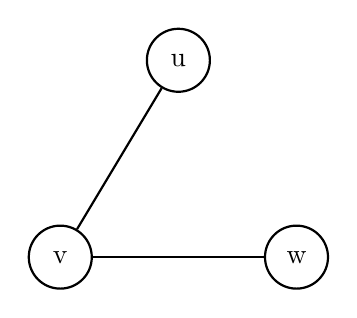
\begin{tikzpicture}[
    vertex/.style={
        circle,
        draw=black,
        thick,
        minimum size=8mm,
        inner sep=0pt
    }
    ]
    \node[vertex] (v) at (0,0) {v};
    \node[vertex] (w) at (3,0) {w};
    \node[vertex] (u) at (1.5, 2.5) {u};

    \draw[thick] (v) -- (u);
    \draw[thick] (v) -- (w);
\end{tikzpicture}}
    \end{minipage}
    \hfill
    \begin{minipage}{0.74\linewidth}
        \resizebox{\linewidth}{!}{\begin{forest}
    % Tree configuration
    for tree={
        circle,
        draw,
        l sep=20pt,
        s sep=15pt,
        edge={Stealth-}
    }
    [$\wedge$, label={[align=center] right: IS di dimensione \\ almeno 2?}
    [$\neg$, label={left: IS?}
    [$\vee$, label={[align=center]left: Entrambi i lati di un \\ arco sono stai scelti?}
    [$\vee$, tier=m2
    [$\wedge$, tier=mid, name=v1
    [u-v, tier=bot, name=d1]
    ]
    [$\wedge$, tier=mid, name=v2
    [u-w, tier=bot, name=d2]
    ]
    ]
    [$\wedge$, tier=mid, name=v3
    [v-w, tier=bot, name=d3]
    ]
    ]
    ]
    [$\vee$, tier=m2, label={[align=center] right: Set di almeno \\ 2 elementi?}
    [$\vee$
    [$\wedge$, tier=b2, name=c1
    [u, tier=bot, name=b1]
    ]
    [$\wedge$, tier=b2, name=c2
    [v, tier=bot, edge={draw=none}, name=b2]
    ]
    ]
    [$\wedge$, tier=b2, name=c3
    [w, tier=bot, name=b3]
    ]
    ]
    ]
    % Draw the arrow using TikZ syntax relative to the forest nodes
    \draw[Stealth-] (v1) to (c1);
    \draw[Stealth-] (v2) to (c2);
    \draw[Stealth-] (v3) to (c3);
    \draw[Stealth-] (c1) to (b2);
    \draw[Stealth-] (c2) to (b1);
    \draw[Stealth-] (c2) to (b3);
    \draw[Stealth-] (c3) to (b2);
    \node[fit=(d1)(d3), label={[align=center]below:$\binom{n}{2}$ input fissi per gli archi \\ (descrizione del grafo)}] {};
    \node[fit=(b1)(b3), label={[align=center]below:$n$ input \\ (nodi nell'IS)}] {};
\end{forest}}
    \end{minipage}
    \caption{Riduzione da 2-IS a CS}
    \label{fig:IStree}
\end{figure}

In Figura \ref{fig:IStree} si può vedere un esempio:
\begin{itemize}
    \item Al di sopra dei nodi di input per $z$, ogni nodo $\wedge$ chiede "sono stati scelti questi due nodi?"; la restante parte destra dell'albero controlla solamente che siano stati scelti almeno due nodi

    \item Il risultato della "scelta" viene messo in $\wedge$ con la codifica degli archi presenti

    \item I risultati vengono messi in $\vee$, quindi risulta 1 se e solo se sono stati scelti due nodi che hanno un arco presente tra loro; viene invertito per avere 1 nel caso di Independent Set

    \item La radice si occupa di controllare che l'input rappresenti un Independent set (sottoalbero di sinistra) di dimensione almeno 2 (sottoalbero di destra)
\end{itemize}

Una volta che abbiamo stabilito che un certo problema è \NPc, possiamo trovarne molti altri usando la seguente osservazione. \\

\begin{fact}
    Se $Y$ è \NPc e $X \in \NP$ è tale che $Y \polred X$, allora anche $X$ è \NPc.
\end{fact}
\begin{proof}
    Sia $Z \in \NP$ qualunque. Allora $Z \polred Y$. Ma dato che $Y \polred X$, allora $Z \polred X$, il che implica che $X$ è \NPc.
\end{proof}

Possiamo subito applicare questa osservazione dimostrando quanto segue. \\

%TODO: cercare dim? Maybe
\begin{theorem}
    CS $\polred$ 3-SAT.
\end{theorem}
\begin{proof}
    Omessa.
\end{proof}

Dato che CS è \NPc, ne segue che anche 3-SAT è \NPc. Ricordando inoltre che 3-SAT $\polred$ Independent Set $\polred$ Vertex Cover $\polred$ Set Cover, ne deduciamo che tutti questi problemi sono \NPc. Al contrario di 3-SAT che è \NPc, 2-SAT (ovvero usando clausole da esattamente due letterali) è un problema risolvibile in tempo lineare.

Si noti che ogni formula booleana può essere equivalentemente rappresentata come un circuito (ovvero un'istanza di CS) o come una formula CNF (ovvero un'istanza di SAT) in modo che tali istanze abbiano lunghezza polinomiale nella lunghezza della formula. Inoltre, ogni istanza $I$ di SAT può essere rappresentata come un'istanza di 3-SAT di lunghezza polinomiale in $|I|$ (queste dimostrazioni sono il processo per la dimostrazione omessa precedentemente).

Al contrario, non è sempre possibile rappresentare una formula booleana in DNF in modo che la DNF abbia lunghezza polinomiale nella lunghezza della formula. Se questo fosse possibile avremmo che $\P \equiv \NP$. La soddisfacibilità di una DNF è decidibile in tempo lineare controllando che esista almeno una congiunzione della formula che è soddisfacibile da un qualche assegnamento.

Si noti che la definizione di $\NP$ è asimmetrica: dato un problema $X = (\I, q) \in \NP$, se $q(I) = 1$ allora esiste un certificato polinomiale $z$ tale che $B(I, z) = 1$ dove $B$ denota il certificatore polinomiale per $X$. Se invece $q(I) = 0$ allora la definizione ci garantisce solo che $B(I,z) = 0$ per un numero esponenziale di certificati $z$. Questa asimmetria si riscontra quanto consideriamo problemi $\bar X = (\I, \bar q)$ che sono complementari di problemi $X = (\I, q)$. Per \textit{complementare} di $X$ si intende che $\bar q(I) = 0$, ma non sappiamo se esista un certificato polinomiale che certifichi $\bar q (I) = 1$. Per esempio, se $X$ è Independent Set, allora per certificare $\bar q(I) = 1$ dovremmo trovare un certificato polinomiale che attesti che il grafo \textbf{non} contenga un insieme indipendente di taglia $k$.

Quindi non è chiaro se $\NP \equiv \coNP$, dove $\coNP$ indica la classe dei problemi di decisione complementari di problemi in $\NP$ (se $\NP$ è l'insieme dei problemi di cui posso verificare una soluzione/certificato in tempo polinomiale, per i problemi in $\coNP$ non è possibile avere una soluzione verificabilemente corretta in tempo polinomiale, è invece possibile verificare in tempo polinomiale che una soluzione restituisce 0).

Lo scenario è differente per $\P$: $X \in \P$ se e solo se $\bar X \in \P$. Infatti $X = (\I, q) \in \P$ implica che esiste un algoritmo per calcolare $q$ in tempo polinomiale. Ma allora si può anche calcolare $\bar q$ in tempo polinomiale semplicemente calcolando $q$ e complementando l'output. Quindi $\P \equiv \coP$.

Dimostrare che $\coNP \not \equiv \NP$ sarebbe un progresso ancora maggiore che dimostrare $\P \not \equiv \NP$. Vale infatti la seguente cosa. \\

\begin{fact}
    Se $\coNP \not \equiv \NP$ allora $\P \not \equiv \NP$.
\end{fact}
\begin{proof}
    Dimostriamo la contrapositiva, ovvero che $\P \equiv \NP$ implica $\coNP \equiv \NP$. Intuitivamente, dato che $\P$ è chiuso rispetto all'operazione di complemento, se $\P \equiv \NP$ allora deve essere che $\coNP \equiv \NP$. Formalmente
    $$ X \in \NP \Longleftrightarrow X \in \P \Longleftrightarrow \bar X \in \P \Longleftrightarrow \bar X \in \NP \Longleftrightarrow X \in \coNP $$
    Il che conclude la dimostrazione.
\end{proof}

Possiamo caratterizzare i problemi $X = (\I, q) \in \coNP$ tramite l'esistenza di un polinomio $p(\cdot)$ e di un certificatore polinomiale $B$, calcolabile in tempo polinomiale, tale che $q(I) = 0$ se e solo se esiste una stringa $z \in \left\{0,1\right\}^{p(|I|)}$ tale che $B(I,z) = 0$. Si noti che $\P \subseteq \coNP$, infatti, potendo implementare $q$ in tempo polinomiale, si può calcolare $B(I,z)$ ignorando $z$ e restituendo $q(I)$.

Una classe particolarmente interessante è quella dei problemi in $\NP \cap \coNP$. Sia $X = (\I, q)$ un tale problema
\begin{itemize}
    \item Dato che $X \in \NP$ esiste un polinomio $p(\cdot)$ e un certificatore polinomiale $B$ tale che $q(I) = 1$ se e solo se esiste una stringa $z \in \left\{0,1\right\}^{p(|I|)}$ tale che $B(I,z) = 1$

    \item Dato che $X \in \coNP$ esiste un polinomio $p'(\cdot)$ e un certificatore polinomiale $B'$ tale che $q(I) = 0$ se e solo se esiste una stringa $z' \in \left\{0,1\right\}^{p'(|I|)}$ tale che $B'(I, z') = 0$
\end{itemize}

Quindi i problemi in $\NP \cap \coNP$ sono tali che per ogni istanza $I$ esiste un certificato polinomiale, sia quando $q(I) = 1$ sia quando $q(I) = 0$.

Si noti che se $X \in \P$ allora $X \in \NP$ ed anche $X \in \coNP$. Quindi $\P \subseteq \NP \cap \coNP$. D'altra parte non si sa se $\P \not \equiv \NP \cap \coNP$. Ovvero non si sa se esistono problemi le cui istanze hanno sempre certificati brevi ma tuttavia non sono risolubili in tempo polinomiale.

% End of np.pdf

    \chapter{Algoritmi Probabilistici}

    % !TeX spellcheck = it_IT
% !TeX root = ../../compl.tex
\section{Algoritmi Montecarlo e Las Vegas}

Un algoritmo probabilistico è un algoritmo che ha accesso a un oracolo che, a ogni chiamata, restituisce in tempo unitario un bit casuale, ovvero una variabile casuale $Y$ tale che $\Pr(Y = 1) = \Pr(Y = 0) = 1/2$. Inoltre, i bit restituiti in una sequenza di chiamate all'oracolo sono indipendenti.

Indicheremo con $Z \in \left\{0,1\right\}^\ast$ la stringa di bit casuali indipendenti che l'oracolo restituisce in una sequenza di chiamate. Indicheremo anche con $A(I, Z) \in \left\{0,1\right\}$ la variabile casuale che rappresenta l'output dell'algoritmo probabilistico $A$ per un problema di decisione $X = (\I, q)$ e avente come input l'istanza $I \in \I$ e i bit casuali $Z$ dell'oracolo. Similmente, indichiamo con $T_A (I, Z)$ la variabile casuale che rappresenta il tempo di esecuzione di $A$ con input $I \in \I$ e bit casuali $Z$ forniti dall'oracolo.

Esistono due principali tipi di algoritmi probabilistici.

\paragraph{Algoritmi Montecarlo.} Sono algoritmi $A$ tali che
\begin{itemize}
    \item Per ogni $I \in \I$, $T_A (I, Z)$ dipende solo da $I$, ovvero il tempo di esecuzione è deterministico

    \item Esiste $I \in \I$ per cui $\Pr \left(A(I, Z) \neq q(I)\right) > 0$, ovvero l'output non è sempre corretto
\end{itemize}

Gli algoritmi Montecarlo si dividono ulteriormente in:
\begin{itemize}
    \item Algoritmi con errore \textbf{one-sided}; un algoritmo ha errore one-sided quando è sempre corretto almeno su uno dei suoi due possibili output. Convenzionalmente, assumeremo che l'algoritmo sia sempre corretto per output 1. In altre parole, $A$ è Montecarlo one-sided quando, per ogni $I \in \I$, $\Pr \left(A(I, Z) = q(I) \mid A(I, Z) = 1\right) = 1$ e $\Pr \left(A(I, Z) = q(I) \mid A(I, Z) = 0\right) > 0$

    \item Algoritmi con errore \textbf{two-sided}. Possono sbagliare su entrambi i possibili output. Ovvero, $A$ è Montecarlo two-sided quando $\Pr\left(A(I,Z) = q(I)\right) > 1/2$ per ogni $I \in \I$
\end{itemize}

Una rappresentazione grafica della relazione fra $q(I)$ e $A(I,Z)$ per un algoritmo Montecarlo one-sided è la seguente
\begin{center}
    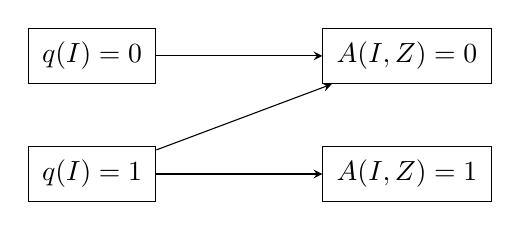
\begin{tikzpicture}[>=stealth]
    % Nodes
    \node[draw, inner sep=5pt] (q0) at (0, 1.5) {$q(I) = 0$};
    \node[draw, inner sep=5pt] (a0) at (4, 1.5) {$A(I, Z) = 0$};
    \node[draw, inner sep=5pt] (q1) at (0, 0)   {$q(I) = 1$};
    \node[draw, inner sep=5pt] (a1) at (4, 0)   {$A(I, Z) = 1$};
    % Arrows connecting the nodes
    \draw[->] (q0) -- (a0);
    \draw[->] (q1) -- (a1);
    \draw[->] (q1) -- (a0);
\end{tikzpicture}
\end{center}

Questo mostra come $A(I,Z) = 1$ può solo corrispondere a $q(I) = 1$, mentre $A(I,Z) = 0$ lascia incertezza sul valore di $q(I)$. Si noti anche che quando $q(I) = 0$ l'algoritmo è sempre corretto.

\paragraph{Algoritmi Las Vegas.} Sono algoritmi che producono sempre l'output corretto ma che hanno un tempo di esecuzione probabilistico (ovvero che dipende dai bit forniti dall'oracolo). Ovvero, un algoritmo $A$ è Las Vegas quando $\Pr\left(A(I,Z) = q(I)\right) = 1$ per ogni $I \in \I$ ma il tempo di calcolo di $A$ su una qualunque istanza $I \in \I$ è una variabile casuale $T_A (I,Z)$ tale che $\Ex\left[T_A (I,Z)\right] < \infty$.

\paragraph{Amplificazione.} Un algoritmo Montecarlo one-sided può essere facilmente trasformato in un algoritmo con probabilità di errore arbitrariamente piccola attraverso un meccanismo di amplificazione

Sia
$$ \Pr \left(A (I, Z) \neq q(I) \mid A(I, Z) = 0 \right) \leq 1 - p_n, \quad \forall I \in \I \text{ con } |I| = n $$
Se su una data istanza l'algoritmo produce 0 in output possiamo eseguirlo nuovamente per amplificare la probabilità di avere l'output corretto. Se $k$ esecuzioni indipendenti producono sistematicamente la risposta 0, allora la probabilità che la risposta corretta sia 1 è al più $\left(1 - p_n\right)^k \leq e^{-p_n k}$. Perché questa probabilità sia al più un $\epsilon > 0$ piccolo a piacere è sufficiente scegliere $k \geq \frac{1}{p_n} \ln \frac{1}{\epsilon}$.

Un meccanismo di amplificazione simile ma leggermente più complesso esiste anche per gli algoritmi Montecarlo two-sided. Supponiamo che su istanze di taglia $n$ l'algoritmo fornisca la risposta errata con probabilità al più $\frac{1}{2} - p_n < \frac{1}{2}$. Per amplificare la probabilità di ottenere la risposta corretta possiamo ripetere l'esecuzione $k$ volte e utilizzare un voto di maggioranza sui $k$ output prodotti (supponiamo, per semplicità, che $k$ sia dispari).

Per analizzare il voto di maggioranza utilizzeremo il seguente lemma. \\

\begin{lemma}[Chernoff-Hoeffding]
    \label{lemma:c-h}
    Siano $Y_1, \dots, Y_k$ variabili casuali Bernoulliane (cioè con valori in $\left\{0,1\right\}$), indipendenti e tali che $\Pr(Y_t = 1) \leq \mu$ per $t = 1, \dots, k$. Allora, per ogni $\epsilon > 0$ fissato
    $$ \Pr \left(\frac{1}{k} \sum_{t=1}^{k} Y_t > \mu + \epsilon\right) \leq e^{-2 \epsilon^2 k} $$
\end{lemma}
\begin{proof}
    Omessa.
\end{proof}

In altre parole, date delle variabili Bernoulliane indipendenti, con limite $\mu$ per il valore atteso, la disuguaglianza stabilisce la probabilità che la media si discosti di una certa quantità ($\epsilon$) dal valore atteso $\mu$. Intuitivamente, rappresenta la probabilità di allontanarsi dal valore atteso all'aumentare del numero di "tentativi" (variabili).

Sia $p_E = \Pr \left(A(I,Z) \neq q(I)\right)$ la probabilità di errore dell'algoritmo su un'istanza $I$ del problema di decisione $(\I, q)$. Siano $X_1, \dots, X_k \in \left\{0,1\right\}$ le variabili casuali indipendenti che denotano gli output prodotti dalle $k$ esecuzioni dell'algoritmo. Sia $M_k \in \left\{0,1\right\}$ la variabile casuale che denota il voto di maggioranza su $X_1, \dots, X_k$ (ovvero $M_k = 1$ se e solo se $\sum_{t=1}^k X_t > \frac{k}{2}$).

Allora
$$ M_k = q(I) \Longleftrightarrow \sum_{t=1}^k Y_t < \frac{k}{2} $$
dove $Y_t = 1$ se e solo se $X_t \neq q(I)$, per $t = 1, \dots, k$ (ovvero, se il risultato della relativa esecuzione dell'algoritmo è sbagliato). In altre parole, il voto di maggioranza $M_k$ è corretto se e solo se l'algoritmo genera output errato in non più di $\left\lfloor\frac{k}{2}\right\rfloor$ delle $k$ esecuzioni.

Ora, $Y_1, \dots, Y_k$ sono variabili casuali indipendenti (perché le esecuzioni dell'algoritmo sono indipendenti), identicamente distribuite, con valori in $\left\{0,1\right\}$ e tali che $\Pr (Y_t = 1) = p_E \leq \frac{1}{2} - p_n$ per ogni $t = 1, \dots, k$.

Applicando il lemma di Chernoff-Hoeffding (\ref{lemma:c-h}) otteniamo che la probabilità che il voto di maggioranza sia sbagliato è limitata da
\begin{align*}
    \Pr \left(\sum_{t=1}^k Y_t > \frac{k}{2}\right) & = \Pr \left(\frac{1}{k} \sum_{t=1}^k Y_t > \frac{1}{2} \right) \\
    & = \Pr \left(\frac{1}{k} \sum_{t=1}^k Y_t > \left(\frac{1}{2} - p_n\right) + p_n \right)  \\
    & \leq \Pr \left(\frac{1}{k} \sum_{t=1}^k Y_t > p_E + p_n \right)  \\
    & \leq e^{-2p_n^2 k}
\end{align*}

Perché la probabilità $e^{-2p_n^2k}$ sia al più un $\epsilon > 0$ piccolo a piacere è sufficiente scegliere
$$k \geq \frac{1}{2p^2_n} \ln \frac{1}{\epsilon}$$

Si noti che nel caso one-sided possiamo usare l'amplificazione per ridurre qualsiasi probabilità di errore strettamente minore di 1, mentre nel caso two-sided la stessa cosa vale per qualsiasi probabilità strettamente minore di $\frac{1}{2}$.

\paragraph{Da Las Vegas a Montecarlo one-sided.} Un algoritmo Las Vegas per un problema di decisione può essere trasformato in un algoritmo Montecarlo one-sided. Per fare ciò utilizziamo la disuguaglianza di Markov. \\

\begin{lemma}[Markov]
    \label{lemma:markov}
    Sia $Z$ una variabile casuale non negativa tale che $\Ex [Z] < \infty$. Allora per ogni $c > 0$
    $$ \Pr (Z > c) \leq \frac{\Ex [Z]}{c} $$
\end{lemma}
\begin{proof}
    Sia $\A$ l'insieme di numeri non negativi tali che $Z \in \A$. Allora
    \begin{align*}
        \Ex[Z] & = \sum_{a \in \A} a \Pr (Z = a) = \overbrace{\sum_{a \in \A: a \leq c} a \Pr(Z = a)}^{\geq 0} + \sum_{a \in \A: a > c} a \Pr (Z = a) \\
        & \geq c \sum_{a \in \A: a > c} \Pr (Z = a) \\
        & = c \Pr (Z = c)
    \end{align*}
    $$ \Ex [Z] \geq c \Pr (Z > c) \implies \Pr (Z > c) \leq \frac{\Ex[Z]}{c} $$
    concludendo la dimostrazione.
\end{proof}

Sia $A$ un algoritmo Las Vegas per un problema di decisione $(\I, q)$. Sia $f: \N \rightarrow \R$ la funzione tale che
$$ f(n) = \max \left\{\Ex \left[T_A (I,Z)\right] \mid I \in \I, \ |I| = n\right\}$$
In altre parole, la funzione rappresenta il massimo del valore atteso per il tempo di esecuzione dell'algoritmo $A$ per istanze di dimensione $n$.

Dato che $A$ è Las Vegas, $f(n) < \infty$ per ogni $n \in \N$. Possiamo quindi trovare una funzione $t: \N \rightarrow \N$ tale che
$$ t(n) \geq \frac{3}{2} f(n), \quad n \in \N $$

Posso quindi costruire un algoritmo $A'$ che simula $A$ sull'istanza $I$ arrestando la simulazione dopo $t(n)$ passi. Se $A$ non ha terminato, allora $A'$ produce 0 in output. Dato che $A$ è Las Vegas, $A'$ sbaglia solo quando $A$ non termina entro $t(n)$ passi. Per la disuguaglianza di Markov, la probabilità che ciò accada è al più
$$ \Pr \left(T_A (I, Z) > t(n)\right) \leq \frac{\Ex \left[T_A (I,Z)\right]}{t(n)} \leq \frac{f(n)}{t(n)} \leq \frac{2}{3} $$

Inoltre, dato che quando $A$ non termina l'output di $A'$ è 0, $A'$ è one-sided dato che l'output 1 è sempre corretto. Quindi $A'$ è un algoritmo Montecarlo one-sided con probabilità di errore al più $2/3$. Infine, si noti che il tempo di esecuzione di $A'$ soddisfa $T_{A'} (I) \leq t(|I|) = \O \left(f(|I|)\right)$.

\vfill

Riassumendo: un algoritmo Las Vegas può diventare Montecarlo one-sided con i seguenti passi
\begin{itemize}
    \item Trova una funzione $t(n)$ che maggiora la funzione $f(n)$, la quale rappresenta il tempo di esecuzione atteso per input di taglia $n$, ovvero $t(n) = m \cdot f(n)$

    \item L'algoritmo Montecarlo usa l'algoritmo Las Vegas, bloccando quest'ultimo se non termina entro $t(n)$ passi; restituisce sempre il risultato dell'algoritmo Las Vegas, oppure 0 se questo non termina

    \item La probabilità di errore è solo nel caso in cui esca 0; per la disuguaglianza di Markov, la probabilità che ciò accada è $\leq \frac{1}{m}$; quando esce 1, l'algoritmo è sempre corretto (quindi one-sided)
\end{itemize}

% end of probAlgo.pdf
    % !TeX spellcheck = it_IT
% !TeX root = ../../compl.tex
\section{Classi di complessità probabilistiche}

Un algoritmo probabilistico per un problema di decisione $X = (\I, q)$ può essere visto come un algoritmo deterministico che ha accesso a una stringa $Z$ di bit casuali. L'algoritmo calcola una funzione $B: \I \times \left\{0,1\right\}^\ast \rightarrow \left\{0,1\right\}$ tale che, per ogni $I \in \I$, $B(I, Z) = q(I)$ con una certa probabilità rispetto all'estrazione della stringa $Z$.

In analogia con la definizione di $\NP$, possiamo definire le classi di problemi di decisione solubili in tempo polinomiale da diversi tipi di algoritmi probabilistici rivisitando la nozione di certificatore polinomiale.

\paragraph{$\BPP$:} La classe di problemi di decisione risolti in modo efficiente da algoritmi Montecarlo two-sided è la classe $\BPP$. Un problema di decisione $X = (\I, q)$ appartiene alla classe $\BPP$ se esiste una funzione $B: \I \times \left\{0,1\right\}^\ast \rightarrow \left\{0,1\right\}$ calcolabile in tempo polinomiale e un polinomio $p(\cdot)$ tali che, per ogni istanza $I \in \I$ essi soddisfano
$$ \Pr \left( B(I,Z) \neq q(I)\right) \leq \frac{1}{3}$$
dove la probabilità è calcolata rispetto all'estrazione di $Z$ con probabilità uniforme da $\left\{0,1\right\}^{p(|I|)}$.

La costante $1/3$ è arbitraria, dato che, come già visto, si può ridurre a piacimento la probabilità di errore di un algoritmo two-sided tramite amplificazione. Una definizione equivalente di $\BPP$ sostituisce la diseguaglianza sopra con
$$ \Pr \left(B(I, Z) \neq q(I)\right) \leq \frac{1}{2} - \frac{1}{p'(|I|)}$$
dove $p'(\cdot)$ è un polinomio. Il meccanismo di amplificazione tramite Lemma di Chernoff-Hoeffding (\ref{lemma:c-h}) implica che è sufficiente eseguire l'algoritmo un numero di volte pari a ordine di $p'(|I|)^2$ per ottenere una probabilità di errore limitata da $1/3$. Dato che $p'(\cdot)$ è un polinomio, l'algoritmo risultante è ancora polinomiale in $|I|$.

In altre parole, $\BPP$ è la classe di algoritmi risolti in modo efficiente da algoritmi Montecarlo two-sided più di metà delle volte, dove la probabilità si può stabilire a piacimento tramite amplificazione rimanendo efficiente.

Si noti che $\P \subseteq \BPP$, dato che avendo un algoritmo polinomiale per calcolare la funzione di decisione $q$ possiamo implementare il certificatore $B$ in tempo polinomiale con probabilità di errore pari a zero. Non è invece noto se $\P \equiv \BPP$, ovvero se ogni algoritmo Montecarlo two-sided possa essere "derandomizzato" in modo da ottenere un algoritmo deterministico polinomiale per lo stesso problema. Non è neanche noto se $\BPP \subseteq \NP$. D'altra parte, dato che la condizione che definisce $\BPP$ è simmetrica rispetto al valore di $q(I)$, ne deduciamo che $\BPP$ è chiusa rispetto al complemento, ovvero $\BPP \equiv \coBPP$.

\paragraph{$\RP$:} La classe di problemi di decisione risolti in modo efficiente da algoritmi Montecarlo one-sided è la classe $\RP$. Un problema di decisione $X = (\I, q)$ appartiene alla classe $\RP$ se esiste una funzione $B: \I \times \left\{0,1\right\}^\ast \rightarrow \left\{0,1\right\}$ calcolabile in tempo polinomiale e un polinomio $p(\cdot)$ tali che, per ogni istanza $I \in \I$
$$
\Pr \left(B(I,Z) = 1\right) \geq \frac{2}{3}, \quad \text{se } q(I) = 1
$$
$$
\Pr \left(B(I,Z) = 0\right) = 1, \quad \text{se } q(I) = 0
$$
dove la probabilità è calcolata rispetto all'estrazione di $Z$ con probabilità uniforme da $\left\{0,1\right\}^{p(|I|)}$.

Si noti che questa definizione corrisponde all'osservazione precedentemente fatta che un algoritmo Montecarlo one-sided è sempre corretto quando $q(I) = 0$. Quando $q(I) = 1$, l'algoritmo è corretto con probabilità almeno $2/3$. Quindi l'algoritmo è sempre corretto su output 1, mentre sbaglia con probabilità al più $1/3$ su output 0. Anche in questo caso la costante $1/3$ è arbitraria grazie al meccanismo di amplificazione.

Possiamo dare una definizione equivalente di $\RP$ sostituendo la prima delle due condizioni con
$$
\Pr \left(B(I,Z) = 1\right) \geq \frac{1}{p'(|I|)}, \quad \text{se } q(I) = 1
$$
dove $p'(\cdot)$ è un polinomio. Il meccanismo di amplificazione implica che è sufficiente eseguire l'algoritmo un numero di volte pari a ordine di $p'(|I|)$ per ottenere una probabilità di errore limitata da $1/3$. Dato che $p'(\cdot)$ è un polinomio, l'algoritmo risultante è ancora polinomiale in $|I|$.

Con un ragionamento simile a quello che ci ha portato a concludere che $\P \subseteq \BPP$, possiamo anche dimostrare che $\P \subseteq \RP$. Ma, a differenza di $\BPP$, questa volta possiamo stabilire una relazione tra $\RP$ e $\NP$. Infatti, la definizione di $\NP$ può essere equivalentemente riscritta nel modo seguente. Un problema di decisione $X = (\I, q)$ appartiene alla classe $\NP$ se esiste una funzione $B: \I \times \left\{0,1\right\}^\ast \rightarrow \left\{0,1\right\}$ calcolabile in tempo polinomiale e un polinomio $p(\cdot)$ tali che, per ogni istanza $I \in \I$, essi soddisfano
$$ \Pr \left(B(I, Z) = 1\right) > 0, \quad \text{se } q(I) = 1 $$
$$ \Pr \left(B(I, Z) = 0\right) = 1, \quad \text{se } q(I) = 0 $$
dove le probabilità sono calcolate rispetto all'estrazione di $Z$ con probabilità uniforme da $\left\{0,1\right\}^{p(|I|)}$.

Dato che per la prima condizione di $\RP$, $\P\left(B(I,Z) = 1\right) \geq \frac{2}{3}$ implica $\P\left(B(I,Z) = 1\right) > 0$, mentre la seconda condizione è uguale nelle due definizioni. Di conseguenza, concludiamo che $\RP \subseteq \NP$. In altre parole, interpretiamo i bit casuali $Z$ nella definizione di $\RP$ come un certificato del fatto che $q(I) = 1$.

La classe $\coRP$ contiene i problemi che sono complementi di problemi in $\RP$. La definizione di $\coRP$ è semplicemente ottenuta invertendo $q(I) = 0$ e $q(I) = 1$ nella definizione di $\RP$. Con una dimostrazione simile a quella di $\RP \subseteq \NP$ possiamo dimostrare che $\coRP \subseteq \coNP$. Come vale $\P \subseteq \RP$ così possiamo dimostrare che $\P \subseteq \coRP$.

Possiamo mettere in relazione $\RP$ e $\coRP$ con $\BPP$ riscrivendo la definizione di quest'ultima come
$$ \Pr \left(B(I, Z) = 1\right) \geq \frac{2}{3}, \quad \text{se } q(I) = 1 $$
$$ \Pr \left(B(I, Z) = 0\right) \geq \frac{2}{3}, \quad \text{se } q(I) = 0 $$
Arrivando così alla conclusione $\RP \subseteq \BPP$ e $\coRP \subseteq \BPP$.

Introduciamo ora la classe $\ZPP \equiv \RP \cap \coRP$. Un problema di decisione $X = (\I, q)$ appartiene alla classe $\ZPP$ se esistono due funzioni $B, B': \I \times \left\{0,1\right\}^\ast \rightarrow \left\{0,1\right\}$ calcolabili in tempo polinomiale e due polinomi $p(\cdot)$, $p'(\cdot)$ tali che, per ogni istanza $I \in \I$, essi soddisfano
$$ \Pr \left(B(I, Z) = 1\right) \geq \frac{2}{3} \ \text{ e } \ \Pr\left(B' (I, Z') = 1\right) = 1 \ \text{se } q(I) = 1 $$
$$ \Pr \left(B(I, Z) = 0\right) \geq \frac{2}{3} \ \text{ e } \ \Pr\left(B' (I, Z') = 0\right) = 1 \ \text{se } q(I) = 0 $$
dove le probabilità sono calcolate rispetto all'estrazione di $Z$ con probabilità uniforme da $\left\{0,1\right\}^{p(|I|)}$ e di $Z'$ con probabilità uniforme da $\left\{0,1\right\}^{p'(|I|)}$.

Non è difficile vedere che la classe $\ZPP$ è la classe dei problemi risolti da algoritmi Las Vegas che terminano in tempo atteso limitato da un polinomio nella lunghezza dell'istanza. Per farlo, abbiamo bisogno del lemma seguente. \\

\begin{lemma}[Valore atteso distribuzione Geometrica]
    \label{lemma:vadg}
    Siano $Z_1, Z_2, \dots$ variabili casuali Bernoulliane, indipendenti e tali che $\Pr(Z_t = 1) = p$ per $t \geq 1$. Sia $G = \min\left\{k \mid Z_k = 1\right\}$. Allora $\Ex [G] = \frac{1}{p}$.
\end{lemma}
\begin{proof}
    \begin{align*}
        \Ex[G] & = \sum_{k=1}^\infty k (1 - p)^{k-1} p
        = p \sum_{k=1}^\infty k (1 - p)^{k-1} \\
        & = -p \sum_{k=1}^\infty \frac{d}{dp} (1 - p)^{k}
        = -p \frac{d}{dp} \sum_{k=1}^\infty (1 - p)^k \\
        & = -p \frac{d}{dp} \left(\frac{1}{1 - (1 - p)} - 1\right)
        = -p \frac{d}{dp} \frac{1 - p}{p} \\
        & = -p \frac{-1}{p^2} = \frac{1}{p}
    \end{align*}
\end{proof}

In altre parole, date delle variabili Bernoulliane indipendenti che restituiscono 1 con probabilità $p$, il valore atteso del numero di variabili da "estrarre" prima del primo 1 è $1/p$.

Ora, se $\X \in \ZPP$ allora posso costruire un algoritmo probabilistico $A$ che, su input $I \in \I$, esegue $B$ e $B'$ arrestandosi non appena $B(I, Z) = 1$ oppure $B'(I, Z') = 0$. In entrambi i casi sappiamo che l'output è corretto, quindi $A$ si arresta sempre con la soluzione corretta. La probabilità che su una particolare istanza $I$ si verifichi $B(I, Z) = 0$ e $B'(I, Z') = 1$ è
\begin{align*}
    \Pr \left(B(I, Z) = 0 \wedge B'(I, Z') = 1\right) & = \Pr \left(B(I, Z) = 0\right) \Pr \left(B'(I,Z') = 1\right) \\
    & \leq \begin{cases}
        \frac{1}{3} \cdot 1 & \text{ se } q(I) = 1 \\
        1 \cdot \frac{1}{3} & \text{ se } q(I) = 0
    \end{cases}
\end{align*}
ovvero al più $1/3$ indipendentemente dal valore di $q(I)$. Quindi la probabilità che $A$ si arresti con la soluzione corretta è almeno $2/3$ in ogni esecuzione di $B$ e $B'$. Usando il lemma sul valore atteso della Geometrica (\ref{lemma:vadg}), il numero atteso di ripetizioni è quindi al più $\frac{3}{2} < 2$. Dato che per ipotesi $B$ e $B'$ terminano entrambe in tempo polinomiale, il tempo atteso di calcolo di $A$ è polinomiale anch'esso.

D'altra parte, sia $A$ un algoritmo Las Vegas per $(\I, q)$ e sia $\mu(I) < p(|I|)$ il valore atteso del tempo di calcolo $T_A (I, Z)$ di $A$ su input $I$. Per la disuguaglianza di Markov (\ref{lemma:markov})
$$ \Pr \left(T_A (I, Z) \geq \left\lceil 3 \mu (I) \right\rceil \right) \leq \frac{1}{3} $$

Quindi se su input $I$ arresto $A$ dopo $\left\lceil 3 \mu (I) \right\rceil$ passi, la probabilità che $A$ non abbia terminato è al più $1/3$. Viceversa, quando $A$ termina l'output è sempre corretto.

Possiamo quindi implementare le funzioni $B$ e $B'$ come segue:
\begin{itemize}
    \item $B$ esegue $A$ e produce 0 se $A$ non termina

    \item Quando $q(I) = 0$ l'output di $B(I,Z)$ è deterministicamente 0

    \item Quando $q(I) = 1$, l'output di $B(I, Z)$ è 1 con probabilità almeno $\frac{2}{3}$

    \item In modo simile possiamo implementare $B'$
\end{itemize}
Dato che $\mu(I) < p(|I|)$, $B$ e $B'$ terminano entrambi in tempo deterministico polinomiale.

Quindi, in particolare, $\ZPP \subseteq \RP$ come avevamo già osservato trasformando un algoritmo Las Vegas in uno Montecarlo one-sided. Ciò implica che risolvere un problema di decisione con un algoritmo Las Vegas è un risultato più forte che risolverlo con un algoritmo Montecarlo (one-sided o two-sided). Infine, dato che $\P$ è incluso sia in $\RP$ che in $\coRP$, abbiamo che $\P \subseteq \ZPP$.

% end RandClasses.pdf
    % !TeX spellcheck = it_IT
% !TeX root = ../../compl.tex
\section{Estrattore di von Neumann}

Un estrattore di causalità è una funzione che trasforma una sorgente non perfettamente casuale in una completamente casuale. Il più semplice estrattore è quello ideato da John von Neumann e risponde alla domanda: \textit{come è possibile usare una moneta truccata per simulare dei lanci di moneta non truccata?}

Più precisamente, avendo una moneta con probabilità sconosciuta $0 < p < 1$ di restituire testa ogni volta che viene lanciata, la si vuole usare per simulare una sequenza di lanci di una moneta equa, ovvero con probabilità $1/2$ di restituire testa.

Siano $X_1, X_2, \dots$ le variabili casuali Bernoulliane indipendenti con $\Pr(X_t = 1) = p$ che modellano i lanci della moneta truccata. Consideriamo le coppe $(X_1, X_2), (X_3, X_4), \dots$ e notiamo che i valori possibili per ogni coppia sono:

\begin{tabular}{c l}
    $(0,0)$ & con probabilità $(1 - p)^2$ \\
    $(1,1)$ & con probabilità $p^2$ \\
    $(0,1)$ e $(1,0)$ & con probabilità $p(1 - p)$
\end{tabular}

Quindi, per ogni coppia $(X_{2k-1}, X_{2k})$ gli eventi $(X_{2k-1}, X_{2k}) = (0,1)$ e $(X_{2k-1}, X_{2k}) = (1,0)$ sono equiprobabili e forniscono la sequenza di lanci desiderata.

\begin{algorithm}[hbt!]
    \caption{Estrattore di von Neumann}
    \KwInput{Sequenza di lanci $X_1, X_2, \dots$}
    \For{$k = 1,2, \dots$}{
        \If{$X_{2k-1} \neq X_{2k}$ \tcp*[r]{Controlla se è una coppia utile}}{
            \eIf{$X_{2k-1} = 1$}{
                Print "Testa" \;
            }{
                Print "Croce" \;
            }
        }
    }
\end{algorithm}

Praticamente, lancia la moneta truccata finché non ottieni due valori diversi di seguito: se il primo dei due è testa, il lancio "equo" è testa, croce altrimenti. Questo funziona in quanto la probabilità che esca $(0,1)$ o $(1,0)$ è la stessa.

Possiamo ora calcolare quanti lanci di moneta truccata servono in media per simulare un lancio di moneta non truccata. Data una sequenza $Z_1, Z_2, \dots$ di variabili Bernoulliane indipendenti tali che $\Pr (Z_k = 1) = q$ per $k \geq 1$, la variabile casuale geometrica $G$ è definita come $G = \min \left\{k = 1,2, \dots \mid Z_k = 1\right\}$.

Chiaramente $\Pr (G = 1) = q$ e $\Pr (G = n) = (1 - q)^{n-1}q$ per ogni $n > 1$. Non è difficile dimostrare che $\Ex [G] = \frac{1}{q}$ (Lemma \ref{lemma:vadg}).

Consideriamo ora la sequenza $Z_1, Z_2, \dots$ di variabili Bernoulliane indipendenti tali che
$$ Z_k = \begin{cases}
    1 & X_{2k-1} \neq X_{2k} \\
    0 & \text{altrimenti}
\end{cases}$$

%TODO:  controlla meglio il calcolo, perché 2?
Per quanto detto prima, $\Pr(Z_k = 1) = 2p(1-p)$. Sia $G$ la variabile geometrica associata alla sequenza delle $Z_k$. Quindi il numero medio di lanci che mi servono è
$$ 2 \Ex [G] = \frac{1}{p (1 - p)} $$

% end vonNeumann.pdf
    % !TeX spellcheck = it_IT
% !TeX root = ../../compl.tex
\section{Il problema del Coupon Collector}

Il problema del coupon collector è definito come segue: sia $X_1, X_2, \dots$ una sequenza di variabili casuali indipendenti e uniformemente distribuite su $n$ valori distinti $a_1, \dots, a_n$
$$ \Pr \left(X_t = a_i \right) = \frac{1}{n}, \quad i = 1, \dots, n, \ \  t \geq 1 $$

Calcolare $\Ex[N]$, dove $N = \min \left\{k \mid \left(\forall i \leq n\right) \left(\exists t \leq k\right) X_t = a_i \right\}$. In altre parole, $N$ è il minimo numero di realizzazioni $x_1, \dots, x_k$ sufficienti a osservare ciascun $a_i$ almeno una volta.

Il nome \textit{coupon collector} deriva dal problema di collezionare tutti gli $n$ possibili coupon contenuti in prodotti da acquistare (per esempio, scatole di cereali), dove ogni scatola contiene uno qualsiasi dei buoni premio con probabilità uniforme.

Un problema equivalente è il seguente: supponiamo che a ogni lancio, una pallina cade con probabilità uniforme in una fra $n$ possibili scatole. Quante palline devo lanciare in media affinché ce ne sia almeno una in ogni scatola?

Un'applicazione concreta del coupon collector è la seguente: supponiamo di voler sapere gli identificativi degli $n$ router attraversati da una sequenza di pacchetti. Mentre non c'è abbastanza spazio in un pacchetto per memorizzare tutti gli $n$ identificativi, è facile memorizzare in un pacchetto l'identificativo di un router a caso tra quelli attraversati. Ci si chiede allora quanti pacchetti servono in media per ottenere gli identificativi di tutti gli $n$ router.

Per analizzare il problema, suddividiamo $X_1, X_2, \dots$ in $n$ blocchi di lunghezze $N_1, \dots, N_n$, dove $N_i$ è il numero di estrazioni aggiuntive che servono per ottenere l'$i$-esimo valore distinto avendone già osservati $i-1$. Quindi
$$ N = \sum_{i=1}^n N_i $$

Le variabili casuali $N_1, \dots, N_n$ sono tutte Geometriche. In particolare, quando $i-1$ valori distinti sono già stati osservati, la probabilità di osservarne uno nuovo è
$$ p_i = 1 - \frac{i - 1}{n} = \frac{n - i + 1}{n} $$

Infatti, $p_1 = 1$ e questo implica $N_1 = 1$ deterministicamente, ovviamente.

Ricordando che il valore atteso di una Geometrica di parametro $p_i$ è $\Ex[N_i] = \frac{1}{p_i}$ (Lemma \ref{lemma:vadg}), per linearità del valore atteso abbiamo
$$ \Ex [N] = \sum_{i=1}^n \Ex [N_i] = \sum_{i=1}^n \frac{1}{p_i} = \sum_{i=1}^n \frac{n}{n - i + 1} = n \sum_{i=1}^n \frac{1}{i} = n \ln n + \Theta (n) $$
dove l'ultima uguaglianza vale perché la somma armonica $1 + \frac{1}{2} + \dots + \frac{1}{n}$ è asintotica a $\ln n + \Theta(1)$.

% end coupon.pdf
    % !TeX spellcheck = it_IT
% !TeX root = ../../compl.tex
\section{Reservoir Sampling}

Si consideri il problema di mantenere una struttura dati che, a ogni istante di tempo, contenga $k$ elementi estratti a caso con probabilità uniforme da uno stream di elementi in ingresso. In particolare, vogliamo sviluppare un algoritmo che soddisfi il seguente invariante: per ogni $t \geq k$, ognuno dei primi $t$ elementi dello stream è contenuto nella struttura dati con probabilità pari a $\frac{k}{t}$.

Per esempio, vogliamo stimare le percentuali delle varie tipologie di oggetti (libri, elettronica, abbigliamento, \dots) venduti su Amazon in un dato lasso di tempo. Se ogni oggetto venduto è campionato con la stessa probabilità, allora la distribuzione delle tipologie nel campiona sarà tendenzialmente uguale a quella nello stream.

Studiamo il problema nel modello streaming: a ogni istante di tempo $t = 1,2, \dots$ l'algoritmo può accedere soltanto al $t$-esimo elemento $x_t$ dello stream. Chiediamo inoltre che l'algoritmo lavori in spazio $\Theta(k)$.

Il seguente algoritmo soddisfa tutte le proprietà richieste.
\begin{algorithm}[h!]
    \caption{Reservoir Sampling}
    \KwInput{Intero $k$}
    $R = \emptyset$ \tcp*[r]{Inizializza la riserva}
    \For{$t = 1,2, \dots$}{
        Leggi il prossimo elemento $x_t$ nello stream\;
        \eIf{$t \leq k$}{
            Aggiungi $x_t$ a $R$\;
        }{
            Con probabilità $\frac{k}{t}$, sostituisci un elemento a caso in $R$ con $x_t$
        }
    }
\end{algorithm}

Nel caso in cui lo stream avesse lunghezza nota $N$, potremmo aggiungere alla riserva ogni elemento dello stream in modo indipendente con probabilità $\frac{k}{N}$. Questo garantirebbe la proprietà che ogni elemento dello stream è contenuto nella riserva con la stessa probabilità, ma il numero di elementi effettivamente inseriti nella riserva potrebbe essere maggiore o minore di $k$. \\

\begin{theorem}
    Sia $R_t$ il contenuto della riserva dopo che sono stati osservati i primi $t$ elementi dello stream. Per ogni $t \geq k$ vale: $\Pr \left(x_i \in R_t \right) = \frac{k}{t}$ per ogni $i \leq t$.
\end{theorem}

Per la dimostrazione useremo più volte il fatto che, per ogni coppia di eventi $A,B$ tale che $\Pr(B) > 0$ vale $\Pr(A \cap B) = \Pr(B) \Pr(A \mid B)$.

\begin{proof}
    La dimostrazione è per induzione su $t \geq k$:
    \begin{itemize}
        \item \textbf{Base:} $t = k$. Allora $\Pr\left(x_i \in R_t\right) = 1 = \frac{k}{t}$ dato che $t = k$

        \item \textbf{Step:} Fissato $t \geq k$, assumiamo l'ipotesi induttiva
        $$ P\left(x_i \in R_t \right) = \frac{k}{t}, \quad \forall i \leq t $$
        e dimostriamo
        $$ \Pr\left(x_i \in R_{t+1}\right) = \frac{k}{t+1}, \quad \forall i \leq t+1 $$
        Se $i = t+1$, allora vale la tesi per costruzione (riga 7 dell'algoritmo). Se invece $i \leq t$, dato che $x_i \in R_{t+1}$ implica $x_i \in R_t$, abbiamo che $\Pr\left(x_i \in R_{t+1}\right) = \Pr \left(x_i \in R_{t+1}, \ x_i \in R_t \right)$. Possiamo quindi scrivere
        \begin{align*}
            \Pr\left(x_i \in R_{t+1}\right) & = \Pr \left(x_i \in R_{t+1}, \ x_i \in R_t \right) \\
            & = \Pr \left(x_i \in R_t \right) \Pr \left(x_i \in R_{t+1} \mid x_i \in R_t \right) \\
            & = \frac{k}{t} \cdot \Pr \left(x_i \in R_{t+1} \mid x_i \in R_t \right) && \text{(per IH)}
        \end{align*}

        Ora si osservi che, dato $x_i \in R_t$, abbiamo che $x_i \notin R_{t+1}$ implica $x_{t+1} \in R_{t+1}$. Quindi possiamo scrivere
        \begin{align*}
            \Pr \left(x_i \in R_{t+1} \mid x_i \in R_t \right) & = 1 - \Pr \left(x_i \notin R_{t+1} \mid x_i \in R_t \right) \\
            & = 1 - \Pr\left(x_i \notin R_{t+1}, \ x_{t+1} \in R_{t+1} \mid x_i \in R_t \right) \\
            & = 1 - \Pr \left(x_{t+1} \in R_{t+1} \mid x_i \in R_t\right) \Pr \left(x_i \notin R_{t+1} \mid x_{t+1} \in R_{t+1}, \ x_i \in R_t \right) \\
            & = 1 - \frac{k}{t+1} \frac{1}{k} \\
            & = \frac{t}{t+1}
        \end{align*}
        dove
        $$ \Pr \left(x_{t+1} \in R_{t+1} \mid x_i \in R_t \right) = \Pr \left(x_{t+1} \in R_{t+1}\right) = \frac{k}{t+1} $$
        per costruzione dell'algoritmo e
        $$ \Pr\left(x_i \notin R_{t+1} \mid x_{t+1} \in R_{t+1}, \ x_i \in R_t \right) = \frac{1}{k} $$
        dato che $x_i$ ha probabilità uniforme di essere selezionato dalla riserva per far posto a $x_{t+1}$. Quindi
        $$ \Pr \left(x_i \in R_{t+1}\right) = \frac{k}{t} \frac{t}{t+1} = \frac{k}{t+1} $$
        che conclude la dimostrazione.
    \end{itemize}
\end{proof}

% end reservoir.pdf






\end{document}
